\documentclass[12pt,a4paper]{report}
\usepackage[utf8]{inputenc}
\usepackage[portuguese]{babel}
\usepackage{amsmath}
\usepackage{amsfonts}
\usepackage{amssymb}
\usepackage{enumitem}
\usepackage{fancyhdr}
\usepackage{geometry}
\usepackage{graphicx}
\usepackage{listings}
\usepackage{multicol}
\usepackage{tcolorbox}
\usepackage{parskip}
\usepackage{setspace}
\usepackage{tikz}
\usepackage{verbatim}
\usepackage{pgfplots}
\pgfplotsset{compat=1.15}
\usepackage{mathrsfs}
\usepackage{tasks}
\usetikzlibrary{arrows, intersections, angles, calc, quotes, babel}

\setstretch{1.2}
\tcbuselibrary{skins, breakable}
\geometry{top=2cm, bottom=2cm, left=2.5cm, right=2.5cm}
\usepackage[colorlinks=true, linkcolor=blue, urlcolor=blue, citecolor=blue]{hyperref}

\pagestyle{fancy}
\fancyhf{}
\fancyhead[C]{\leftmark}
\fancyfoot[C]{\thepage}

% Estilo de caixa para destaque conceitual com quebra de página
\newtcolorbox{destaque}[1][]{
	enhanced,
	breakable,
	colback=gray!5,
	colframe=black!70,
	boxrule=1pt,
	arc=4pt,
	left=10pt,
	right=10pt,
	top=8pt,
	bottom=8pt,
	fonttitle=\bfseries,
	title=#1
}

\begin{document}
	
	\begin{titlepage}
		\centering
		
		% --- Cabeçalho da Instituição ---
		\includegraphics[width=8cm]{../alexjordane.github.io/ifes.png}\\[1cm]
		
		{\Large \textbf{Instituto Federal do Espírito Santo}}\\[0.5cm]
		{\large \textbf{Licenciatura em Matemática $\bullet$ Educimat}}\\[0.5cm]
		
		\vspace{\fill}
		
		% --- Título ---
		{\Huge \textbf{Fractais de Sierpinski}}\\[0.4cm]
		{\LARGE \textbf{Roteiro de Construção no GeoGebra}}\\[0.5cm]
		{\Large Material Teórico e Metodológico de Apoio}
		
		\vspace{\fill}
		
		% --- Autoria ---
		{\Large Professor Alex Jordane}
		
		\vspace{\fill}
		
		% --- Local e Data ---
		{\large Vitória -- ES}\\[0.2cm]
		{\large 2026}
		
	\end{titlepage}
	
	\setcounter{page}{1}
	
	\chapter*{Apresentação}
	\thispagestyle{empty}
	
	Neste material, apresentamos um roteiro prático e conceitual para a construção de fractais clássicos de Wacław Sierpiński utilizando o software de geometria dinâmica \textbf{GeoGebra}: o \textbf{Triângulo de Sierpinski} (no plano), a \textbf{Pirâmide de Sierpinski} (no espaço tridimensional) e o \textbf{Tapete de Sierpinski}.
	
	Ao longo dos capítulos, exploramos como transformações geométricas de \textbf{homotetia}, combinadas ao achatamento estrutural de listas aninhadas (\texttt{Nivelar}) e a processos recursivos controlados por parâmetros dinâmicos (\texttt{ControleDeslizante} e \texttt{Iteração}), permitem modelar e visualizar a autossimilaridade característica da geometria fractal.
	
	Bons estudos!
	
	\vspace{\fill}
	
	{\footnotesize
		\texttt{Material elaborado em setembro de 2026.}\\
		\texttt{Elaborado em colaboração com a inteligência artificial Gemini.}\\
		\texttt{O compartilhamento e a reprodução deste material são permitidos para fins didáticos, desde que citadas a fonte e a autoria.}\\
		\texttt{Esta obra está sob uma Licença Creative Commons Atribuição-NãoComercial-SemDerivações 4.0 Internacional.}
		\begin{center}
			\includegraphics[width=3.5cm]{../alexjordane.github.io/CC.png}
		\end{center}
	}
	
	\tableofcontents
	\thispagestyle{empty}
	
	\vspace{1cm}
	
	\chapter{Triângulo de Sierpinski}
	\label{cap:triangulo}
	
	\begin{center}
		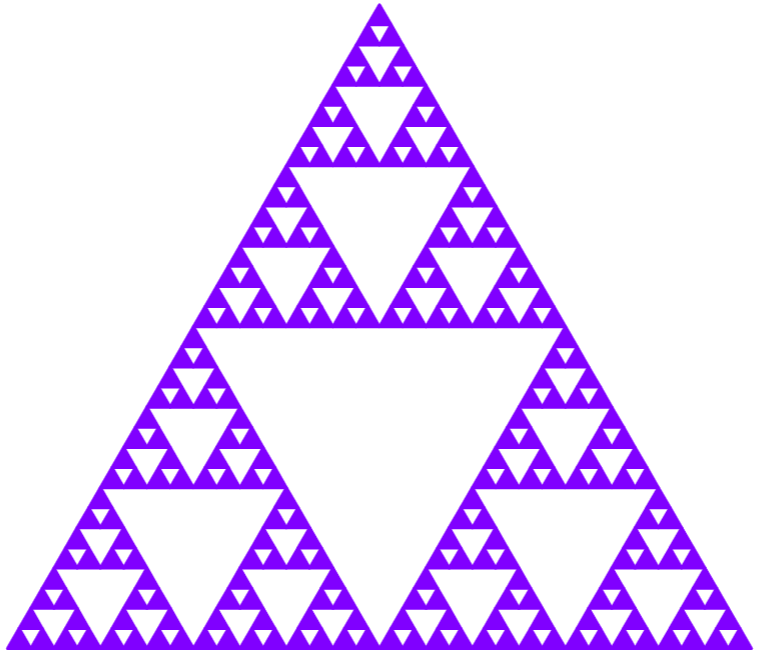
\includegraphics[width=0.7\linewidth]{Triangulo}
	\end{center}
		
	\section{Triângulo inicial ($t_1$)}
	\begin{enumerate}
		\item \texttt{A = (0, 0)}
		\item \texttt{B = (2, 0)}
		\item \texttt{C = (1, $\sqrt{3}$)}
		\item \texttt{t1 = Polígono(A, B, C)}
	\end{enumerate}
	
	Os pontos $A$, $B$ e $C$ podem ter quaisquer coordenadas. Iniciamos com essas coordenadas para termos um triângulo equilátero.
	
	Chamamos o triângulo inicial de $t1$, mas podemos usar o nome que quisermos.
	
	\section{O primeiro triângulo com vértice em $A$}
	
	Neste caso vamos gerar uma figura homotética a $t1$, com razão de $0.5$ e tendo $A$ como ponto central. Esse triângulo é somente um teste para entendermos como funciona o comando \texttt{Homotetia}. Ele pode ser apagado do nosso desenho.
	
	O comando fica da seguinte forma:
	
	\begin{enumerate}[resume]
		\item \texttt{Homotetia(t1, 0.5, A)}
	\end{enumerate}
	
	\subsection{Sintaxe do comando \texttt{Homotetia}}
	
	\begin{destaque}[Comando \texttt{Homotetia}]
		\begin{verbatim}
Homotetia(<Objeto>, <Razao de Dilatacao>, <Ponto Central>)
Homotetia(<Objeto>, <Razao de Dilatacao>)
		\end{verbatim}
		
		\textbf{Parâmetros Operacionais:}
		\begin{itemize}
			\item \textbf{\texttt{<Objeto>}:} objeto a ser submetido à homotetia. O argumento admite tipos como ponto, segmento, reta, polígono 2D, poliedro 3D ou listas heterogêneas contendo esses tipos.
			\item \textbf{\texttt{<Razão de Homotetia>}:} razão que define o fator multiplicativo afim da transformação. Pode ser uma constante algébrica, uma expressão escalar ou uma variável dinâmica vinculada a um controle deslizante.
			\item \textbf{\texttt{<Ponto Central>}:} ponto que atua como o centro de contração/expansão. Caso o parâmetro seja omitido, o software adota a origem canônica do sistema de coordenadas: $(0,0)$ em $\mathbb{R}^2$ ou $(0,0,0)$ em $\mathbb{R}^3$.
		\end{itemize}
	\end{destaque}
	
	\section{A primeira etapa do Triângulo de Sierpinski}
	
	Vamos usar o comando \texttt{Homotetia} três vezes. A primeira com centro em $A$, a segunda com centro em $B$ e finalmente a terceira com centro em $C$. 
	
	\subsection{Com três comandos}
	
	Podemos fazer isso com três comandos:
	
	\begin{enumerate}[start=5]
		\item \texttt{Homotetia(t1, 0.5, A)}
		\item \texttt{Homotetia(t1, 0.5, B)}
		\item \texttt{Homotetia(t1, 0.5, C)}
	\end{enumerate}
	
	\subsection{Usando o comando \texttt{Nivelar}}
	
	Mas também podemos fazer isso com uma única linha de comando, usando o comando \texttt{Nivelar}:
	
	\begin{enumerate}[start=5]
		\item \texttt{Etapa1 = Nivelar(\{Homotetia(t1, 0.5, A), Homotetia(t1, 0.5, B), \\Homotetia(t1, 0.5, C)\})}
	\end{enumerate}
	
	\begin{destaque}[O Comando \texttt{Nivelar} no GeoGebra]
		Em ambientes de geometria dinâmica e sistemas de álgebra computacional como o GeoGebra, uma lista é formalmente definida como uma sequência ordenada de elementos, denotada por $\mathcal{L} = \{x_1, x_2, \dots, x_k\}$. Quando os próprios elementos $x_i$ constituem listas, estabelece-se uma estrutura hierárquica aninhada (ou árvore de listas), que pode ser compreendida como uma família de conjuntos:
		\[
		\mathcal{L}_{\text{aninhada}} = \{\mathcal{L}_1, \mathcal{L}_2, \dots, \mathcal{L}_m\} = \big\{\{y_{1,1}, \dots, y_{1,k_1}\}, \dots, \{y_{m,1}, \dots, y_{m,k_m}\}\big\}.
		\]
		
		O comando \texttt{Nivelar} (\textit{Flatten}, na sintaxe original em inglês) implementa uma operação de achatamento estrutural, realizando a união linearizada de todas as sublistas em um único nível de indexação:
		\[
		\operatorname{Nivelar}(\mathcal{L}_{\text{aninhada}}) = \{y_{1,1}, \dots, y_{1,k_1}, y_{2,1}, \dots, y_{2,k_2}, \dots, y_{m,1}, \dots, y_{m,k_m}\}.
		\]
		
		Isso faz com que a lista \texttt{Etapa1} se constitua de apenas uma lista simples e facilita o processamento no GeoGebra. Em alguns testes que fizemos, o GeoGebra encontrou dificuldades em dar continuidade aos processos sem esse \textbf{nivelamento}.
	\end{destaque}
	
	\section{As próximas etapas do Triângulo de Sierpinski}
	
	Daqui em diante já podemos ampliar para as próximas etapas. A ideia é que a \texttt{Etapa2} use como referência a \texttt{Etapa1}, e não mais o $t1$. Consequentemente, a \texttt{Etapa3} use como referência a \texttt{Etapa2}, e assim sucessivamente até quando quisermos!
	
	\begin{enumerate}[resume]	
		\item \texttt{Etapa2 = Nivelar(\{Homotetia(Etapa1, 0.5, A), Homotetia(Etapa1, 0.5, B), 
			Homotetia(Etapa1, 0.5, C)\})}
			
		\item \texttt{Etapa3 = Nivelar(\{Homotetia(Etapa2, 0.5, A), Homotetia(Etapa2, 0.5, B), 
			Homotetia(Etapa2, 0.5, C)\})}
			
		\item \texttt{Etapa4 = Nivelar(\{Homotetia(Etapa3, 0.5, A), Homotetia(Etapa3, 0.5, B), 
			Homotetia(Etapa3, 0.5, C)\})}
	\end{enumerate}
	
	\section{Sierpinski por Iteração}
	
	Vamos agora para o momento final, em que implementaremos a ideia de recursividade e um controle de nível.
		
	\subsection{Controle deslizante}
	
	\begin{enumerate}[start=5]
		\item \texttt{n = ControleDeslizante(0, 6, 1)}
	\end{enumerate}
	
	O comando \texttt{ControleDeslizante} cria uma variável no GeoGebra que se apresenta na tela como uma barrinha que pode ter seu valor alterado. A sintaxe é complexa, mas vamos simplificá-la a três parâmetros:
	
	\begin{itemize}
		\item \textbf{\texttt{<Mínimo>}:} valor numérico mínimo ($0$) que a variável pode receber. É o limite inferior do controle deslizante.
		\item \textbf{\texttt{<Máximo>}:} valor numérico máximo ($6$) que a variável pode receber. É o limite superior do controle deslizante.
		\item \textbf{\texttt{<Incremento>}:} define o valor do incremento ($1$) no controle deslizante.
	\end{itemize}
	
	No nosso caso, o controle deslizante (ou a variável) $n$ varia de $0$ a $6$, de $1$ em $1$, ou seja, $n \in \{0, 1, 2, 3, 4, 5, 6\}$.
	
	\subsection{O comando \texttt{Iteração}}
	
	\begin{enumerate}[resume]
		\item \texttt{Sierpinski = Iteração(Nivelar(\{Homotetia(L, 0.5, A), Homotetia(L, 0.5, B), 
				Homotetia(L, 0.5, C)\}), L, \{\{t1\}\}, n)}
	\end{enumerate}
	
	O comando \texttt{Iteração} permite criar processos recursivos que se repetem quantas vezes desejarmos. Vamos usar a forma ampliada deste comando:
	
	\begin{destaque}[Comando \texttt{Iteração}]
		\begin{verbatim}
Iteração(<Expressão>, <Variável>, <Valor Inicial>, <Número de Iterações>)
		\end{verbatim}
		
		\textbf{Parâmetros Operacionais:}
		\begin{itemize}
			\item \texttt{<Expressão>}: A lei de transformação que gera a próxima etapa a partir da etapa anterior (por exemplo, uma expressão envolvendo homotetias ou rotações combinadas com \texttt{Nivelar}).
			\item \texttt{<Variável>}: O símbolo literal (como \texttt{L}, \texttt{P} ou \texttt{x}) que atua formalmente como o argumento da transformação, representando a saída do passo anterior que alimenta o passo seguinte.
			\item \texttt{<Valor Inicial>}: O objeto de partida (um número, um ponto ou uma lista de polígonos, como \texttt{\{\{t1\}\}} ou \texttt{\{A\}}).
			\item \texttt{<Número de Iterações>}: O valor inteiro $n$ que define a quantidade de aplicações sucessivas da expressão.
		\end{itemize}
	\end{destaque}
	
	Em nosso caso, no comando \texttt{Sierpinski = Iteração(Nivelar(\{Homotetia(L, 0.5, A), Homotetia(L, 0.5, B), Homotetia(L, 0.5, C)\}), L, \{\{t1\}\}, n)}, temos os seguintes parâmetros:
	
	\begin{itemize}
		\item \texttt{<Expressão> = Nivelar(\{Homotetia(L, 0.5, A), Homotetia(L, 0.5, B), Homotetia(L, 0.5, C)\})}: significa que o GeoGebra irá repetir esse comando completo $n$ vezes. Aqui é importante notar que não usamos mais $t1$, mas $L$, isso porque a primeira iteração (etapa) irá acontecer com $t1$, mas a segunda com a primeira e assim sucessivamente.
		\item \texttt{<Variável> = L}: indica o que será alterado na \texttt{<Expressão>} a cada iteração. 
		\item \texttt{<Valor Inicial> = \{\{t1\}\}}: começamos a iteração com $t1$.
		\item \texttt{<Número de Iterações>}: usamos a variável (controle deslizante) $n$ como valor para a quantidade de iterações.
	\end{itemize}
	
	\section{Configurações de Estilo}
	
	Além da construção, seguem algumas configurações que embelezam o nosso triângulo. Para isso, clique com o botão direito no objeto \texttt{Sierpinski}, acesse \textbf{Configurações} e altere os itens a seguir:
	
	\subsection{Aba Estilo}
	
	\begin{itemize}
		\item \textbf{Opacidade do Traço}: \texttt{0}\% (faz com que o contorno do triângulo fique completamente transparente).
	\end{itemize}		
	
	\subsection{Aba Avançado -- Cores Dinâmicas (HSV)}
	
	\begin{itemize}
		\item \textbf{Matiz}: \texttt{NúmeroAleatório(n, 100) / 100} (faz com que a cor do triângulo seja escolhida no intervalo $\left[\dfrac{n}{100}, 1\right]$).
		\item \textbf{Saturação}: \texttt{1}
		\item \textbf{Valor}: \texttt{1}
		\item \textbf{Transparência}: \texttt{1} (faz com que o preenchimento do triângulo fique completamente opaco).
	\end{itemize}
	
	\chapter{Pirâmide de Sierpinski}
	\label{cap:piramide}
	
	\begin{center}
		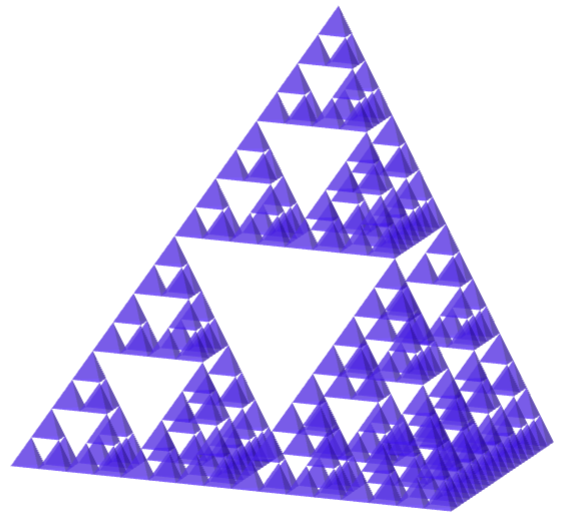
\includegraphics[width=0.7\linewidth]{Piramide}
	\end{center}
	
	\section{Pirâmide inicial ($p_1$)}
	\begin{itemize}
		\item \texttt{A = (0, 2, 0)}
		\item \texttt{B = ($-\sqrt{3}$, -1, 0)}
		\item \texttt{C = ($\sqrt{3}$, -1, 0)}
		\item \texttt{D = (0, 0, $2\sqrt{2}$)}
		\item \texttt{p1 = Pirâmide(A, B, C, D)}
	\end{itemize}
	
	\section{Controle deslizante}
	\texttt{n = ControleDeslizante(0, 4, 1)}
	
	Optamos por limitar o controle deslizante a $4$ para não deixar a construção lenta, pois a renderização tridimensional exige maior processamento.
	
	\section{Pirâmide de Sierpinski por Etapas}
	\begin{destaque}[Construção por Etapas Sucessivas]
		\begin{verbatim}
E1 = Nivelar({Homotetia(p1, 0.5, A), Homotetia(p1, 0.5, B), 
    Homotetia(p1, 0.5, C), Homotetia(p1, 0.5, D)})
    
E2 = Nivelar({Homotetia(E1, 0.5, A), Homotetia(E1, 0.5, B), 
    Homotetia(E1, 0.5, C), Homotetia(E1, 0.5, D)})
    
E3 = Nivelar({Homotetia(E2, 0.5, A), Homotetia(E2, 0.5, B), 
    Homotetia(E2, 0.5, C), Homotetia(E2, 0.5, D)})
		\end{verbatim}
	\end{destaque}
	
	\section{Pirâmide de Sierpinski por Iteração}
	\begin{destaque}[Construção Recursiva com \texttt{Iteração}]
		\begin{verbatim}
Sierpinski = Iteração(Nivelar({Homotetia(L, 0.5, A), Homotetia(L, 0.5, B), 
    Homotetia(L, 0.5, C), Homotetia(L, 0.5, D)}), L, {{p1}}, n)
		\end{verbatim}
	\end{destaque}
	
	\chapter{Tapete de Sierpinski}
	\label{cap:tapete}
	
	\begin{center}
		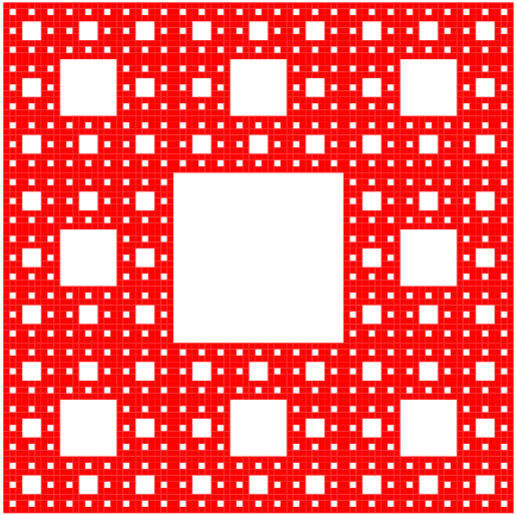
\includegraphics[width=0.7\linewidth]{Tapete}
	\end{center}
		
	O Tapete de Sierpinski segue o mesmo princípio recursivo do triângulo, porém a figura inicial é um quadrado dividido em 9 subquadrados congruentes (razão de homotetia $\frac{1}{3}$), mantendo-se os 8 quadrados periféricos (nos 4 vértices e nos 4 pontos médios dos lados) e removendo-se o quadrado central.
	
	\section{Quadrado inicial ($q_1$)}
	\begin{enumerate}
		\item \texttt{A = (0, 0)}
		\item \texttt{B = (2, 0)}
		\item \texttt{C = (2, 2)}
		\item \texttt{D = (0, 2)}
		\item \texttt{q1 = Polígono(A, B, C, D)}
	\end{enumerate}
	
	\section{Controle deslizante}
	\begin{enumerate}[resume]
		\item \texttt{n = ControleDeslizante(0, 3, 1)}
	\end{enumerate}
	
	\section{Tapete de Sierpinski por Iteração}
	\begin{enumerate}[resume]
		\item Comando recursivo aplicando 8 homotetias de razão $\frac{1}{3}$ (centradas nos vértices $A, B, C, D$ e nos pontos médios dos lados):
	\end{enumerate}
	\begin{destaque}[Construção Recursiva do Tapete de Sierpinski]
		\begin{verbatim}
Sierpinski = Iteração(Nivelar({Homotetia(L, 1/3, A), 
    Homotetia(L, 1/3, B), Homotetia(L, 1/3, C), Homotetia(L, 1/3, D),
    Homotetia(L, 1/3, (A+B)/2), Homotetia(L, 1/3, (B+C)/2), 
    Homotetia(L, 1/3, (C+D)/2), Homotetia(L, 1/3, (D+A)/2)}), 
    L, {{q1}}, n)
		\end{verbatim}
	\end{destaque}

\end{document}
